\section{Where We Left Off}


\begin{frame}{Unfinished Business from Lecture 6}
    Delivery time data, $n=25$, $p=3$: $\hat y = 2.341 + 1.616\,x_1 + 0.0144\,x_2$, with $x_1$ = cases and $x_2$ = distance (ft).
    \svspace{0.5em}
    \begin{itemize}
        \item Lecture 6 singled out observation 9 (30 cases, 1460 ft): leverage $h_{99}=0.498$, studentized residual $r_9=3.214$, R-student $t_9=4.311$.
        \item Residual analysis asked whether the \emph{model as a whole} is adequate. It told us that observation 9 is unusual.
        \item It did not tell us whether observation 9 \emph{changes our conclusions}, or whether it is a ``real'' outlier rather than chance. Lecture 6 left the outlier test for later.
    \end{itemize}
    \svspace{0.5em}
    This lecture: how unusual is a point, and how much does the fit depend on it?
\end{frame}


\begin{frame}{One Delivery Out of 25}
    Fit the model twice, with and without observation 9:
    \begin{center}
        \small
        \begin{tabular}{lrrr}
            \toprule
            & $\hat\beta_0$ & $\hat\beta_1$ (cases) & $\hat\beta_2$ (distance) \\
            \midrule
            All 25 observations & 2.341 & 1.616 & 0.0144 \\
            Without observation 9 & 4.447 & 1.498 & 0.0103 \\
            \bottomrule
        \end{tabular}
    \end{center}
    \begin{itemize}
        \item The distance effect drops by 28\%, more than one standard error ($0.0041$ against $\se(\hat\beta_2)=0.0036$).
        \item One delivery out of 25 moves a conclusion that a $t$-test called highly significant ($p=0.0006$).
    \end{itemize}
    We need tools that find such points \emph{without} refitting the model $n$ times by hand.
\end{frame}


\begin{frame}{Data in This Lecture}
    \begin{itemize}
        \item \textbf{Delivery time} (MPV Example 3.1; diagnostics in MPV Chapter 6): $y$ = time (min) to stock a vending machine, $x_1$ = cases stocked, $x_2$ = distance walked (ft), $n=25$.
        \begin{itemize}
            \item Typical route: about 9 cases and 400 ft.
            \item Observation 9: 30 cases, 1460 ft, 79.24 min. Observation 22: 26 cases, 810 ft, 52.32 min. These are the two largest values of \emph{both} regressors; next come 17 cases and 776 ft.
        \end{itemize}
        \item \textbf{Simulated data}: 18 points on a straight line plus one extra point, placed in four different ways to show the four kinds of unusual point.
    \end{itemize}
    \svspace{0.3em}
    MPV = Montgomery, Peck \& Vining, \emph{Introduction to Linear Regression Analysis}, 5th ed.
\end{frame}


\section{Outliers, Leverage and Influence}


\begin{frame}{Why Least Squares Is Sensitive}
    Least squares minimizes $\sum_i e_i^2$: every residual is \emph{squared} before it is counted.
    \svspace{0.5em}
    \begin{itemize}
        \item A residual of 10 costs $100$, as much as a hundred residuals of size 1.
        \item So the fitted surface bends a long way to shrink one large residual, even if that makes many small residuals a little larger.
        \item One discordant point can therefore move the whole fit. Whether it does depends on \emph{where} the point is, not only on how far it is from the surface.
    \end{itemize}
\end{frame}


\begin{frame}{Three Different Ways to Be Unusual}
    \begin{itemize}
        \item \textbf{Outlier}: $y_i$ is unusual \emph{given} its $\bx_i$. It lies far from the fitted surface: a large residual.
        \item \textbf{High-leverage point}: $\bx_i$ is unusual. It lies far from the other points in the space of the regressors, whatever its $y_i$.
        \item \textbf{Influential point}: removing it changes the fit noticeably: the coefficients, the fitted values, or their standard errors.
    \end{itemize}
    \svspace{0.5em}
    The first two describe the point. The third describes what the point \emph{does} to the model. Neither an outlier nor a high-leverage point has to be influential.
\end{frame}


\begin{frame}{Influence = Push $\times$ Lever Arm}
    \textbf{A seesaw.} In simple regression the least-squares line always passes through $(\bar x,\bar y)$. Think of that point as the pivot of a seesaw.
    \svspace{0.3em}
    \begin{itemize}
        \item The \textbf{residual} is how hard a point pushes the line up or down.
        \item The \textbf{leverage} is how far from the pivot it sits: its lever arm.
        \item The \textbf{influence} is the turning effect: a push at the pivot barely tilts the line; the same push at the end of the seesaw tilts it a lot.
    \end{itemize}
    \svspace{0.3em}
    Later in the lecture this becomes a formula: Cook's distance is (size of residual) $\times$ (leverage factor).
\end{frame}


\begin{frame}{The Seesaw Picture}
    \begin{center}
        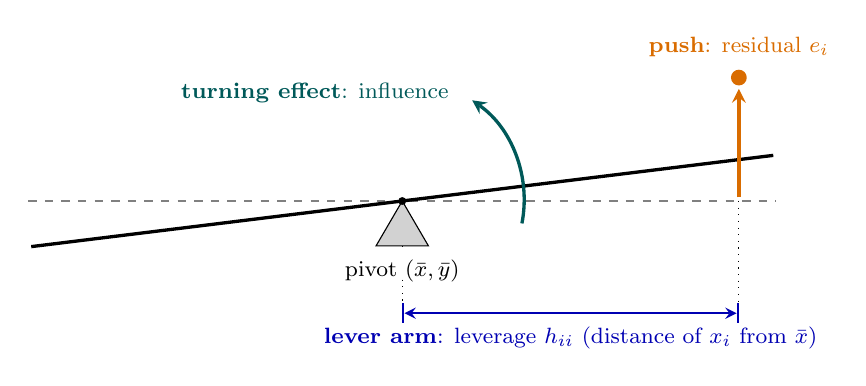
\begin{tikzpicture}[scale=0.95, >=stealth, every node/.style={font=\footnotesize}]
            % fit without the point (dashed) and fit pulled by the point (solid, turned about the pivot)
            \draw[dashed, gray] (-5,0) -- (5,0);
            \draw[very thick] (-4.96,-0.61) -- (4.96,0.61);
            % pivot at (x-bar, y-bar)
            \fill[gray!35] (0,0) -- (-0.35,-0.6) -- (0.35,-0.6) -- cycle;
            \draw (0,0) -- (-0.35,-0.6) -- (0.35,-0.6) -- cycle;
            \fill (0,0) circle (1.5pt);
            \node[anchor=north] at (0,-0.65) {pivot $(\bar x,\bar y)$};
            % push: the residual
            \draw[->, very thick, orange!85!black] (4.5,0.05) -- (4.5,1.5);
            \fill[orange!85!black] (4.5,1.65) circle (3pt);
            \node[anchor=south, orange!85!black] at (4.5,1.8) {\textbf{push}: residual $e_i$};
            % lever arm: the leverage
            \draw[dotted] (4.5,0) -- (4.5,-1.5);
            \draw[dotted] (0,-0.6) -- (0,-0.68);
            \draw[dotted] (0,-1.05) -- (0,-1.5);
            \draw[|<->|, thick, blue!70!black] (0,-1.5) -- (4.5,-1.5);
            \node[anchor=north, blue!70!black] at (2.25,-1.55) {\textbf{lever arm}: leverage $h_{ii}$ (distance of $x_i$ from $\bar x$)};
            % turning effect: the influence
            \draw[->, very thick, teal!70!black] (1.6,-0.3) arc[start angle=-11, end angle=55, radius=1.63];
            \node[anchor=east, teal!70!black] at (0.75,1.45) {\textbf{turning effect}: influence};
        \end{tikzpicture}
    \end{center}
    \begin{itemize}
        \item Dashed: the fit without the point. Solid: the point lifts the far end, and the line turns about the pivot.
        \item Move the same point to $\bar x$: it lifts the whole line a little but cannot turn it, since its lever arm is zero.
    \end{itemize}
\end{frame}


\begin{frame}{The Four Cases}
    \begin{columns}[T]
        \begin{column}{0.34\textwidth}
            \footnotesize
            One extra point (orange) placed four ways; solid line with it, dashed without.
            \begin{itemize}
                \item[(a)] At $\bar x$, on the line: nothing happens.
                \item[(b)] At $\bar x$, far above: the line lifts a little; the slope does not change.
                \item[(c)] Far from $\bar x$, on the line: slope $1.390\to1.397$.
                \item[(d)] Far from $\bar x$, off the line: slope $1.390\to0.323$. One point overrules 18.
            \end{itemize}
        \end{column}
        \begin{column}{0.66\textwidth}
            \centering
            % Figure: influence-geometry.pdf (see influence-geometry.R)
            \mode<presentation>{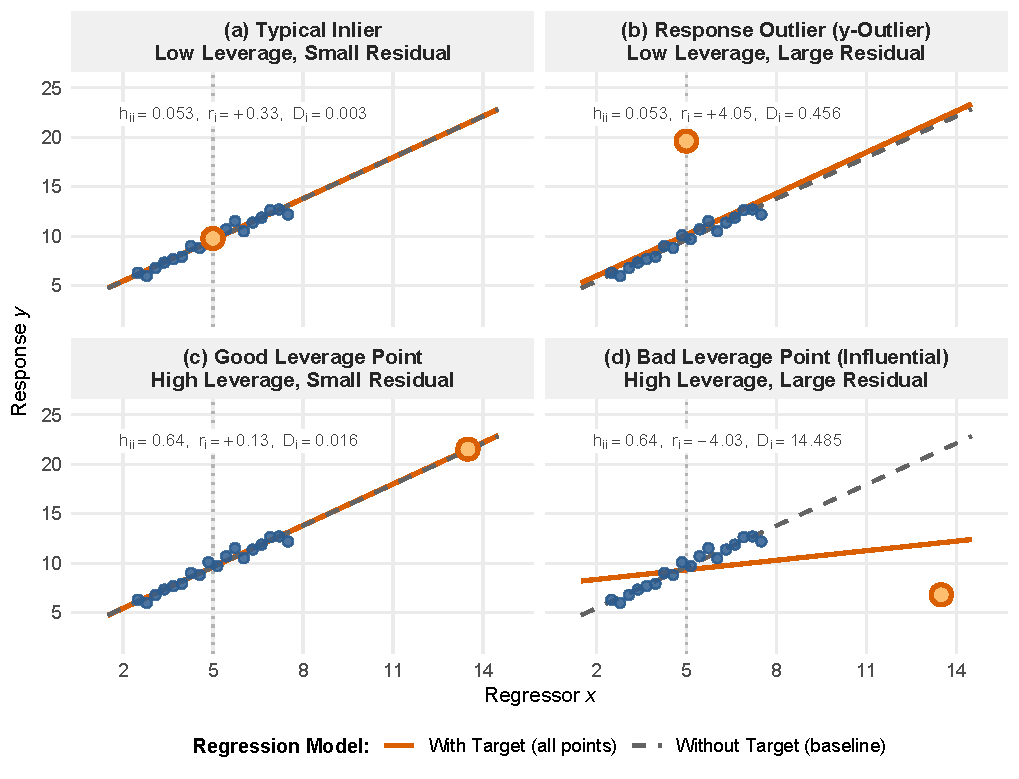
\includegraphics[height=0.8\textheight,width=\linewidth,keepaspectratio]{figures/influence-geometry.pdf}}
            \mode<article>{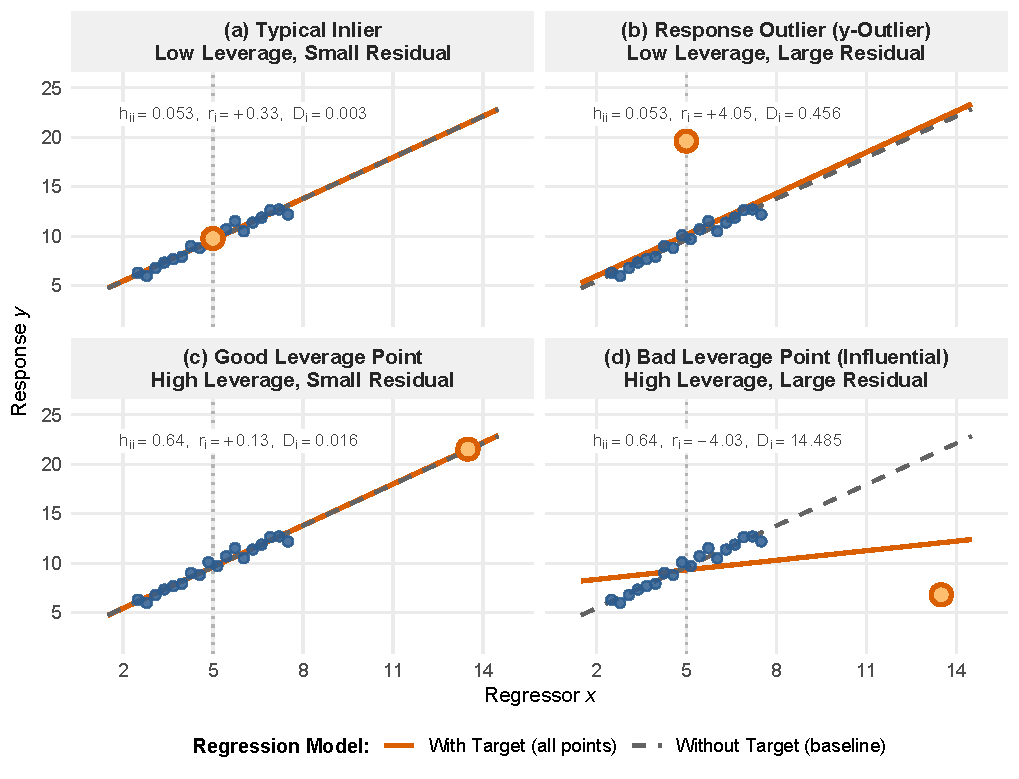
\includegraphics[width=0.8\linewidth]{figures/influence-geometry.pdf}}
        \end{column}
    \end{columns}
\end{frame}


\begin{frame}{Question: Is a High-Leverage Point Bad?}
    \begin{itemize}
        \item In panel (c) the extra point has the same high leverage as in (d), yet the fit hardly changes. Is it harmful, harmless, or helpful?
        \item Panel (b) has a large residual. Why does it not tilt the line?
    \end{itemize}
    % Answer:
    % - (c) is helpful: it agrees with the trend and stretches the range of x, so S_xx grows and Var(slope) = sigma^2/S_xx shrinks. A "good" leverage point.
    % - (b) sits at the pivot x_bar: its push has no lever arm. It lifts the line (intercept) but cannot turn it.
    % - Leverage is potential influence. It becomes actual influence only when the response disagrees with the rest of the data, as in (d).
\end{frame}


\section{Leverage}


\subsection{The Hat Matrix Diagonal}


\begin{frame}{Leverage Revisited}
    From Lecture 6: $\hat{\by}=\bH\by$ with $\bH=\bX(\bX'\bX)^{-1}\bX'$, and the leverage of observation $i$ is
    \[
    h_{ii}=\bx_i'(\bX'\bX)^{-1}\bx_i,
    \qquad
    \hat y_i = h_{ii}\,y_i+\sum_{j\ne i}h_{ij}\,y_j .
    \]
    \begin{itemize}
        \item $h_{ii}=\partial\hat y_i/\partial y_i$: if $y_i$ goes up by one unit, its own fitted value goes up by $h_{ii}$ units.
        \item So $h_{ii}$ is the \emph{share of the say} that observation $i$ has in its own fitted value. The rest comes from its neighbours.
        \item Observation 9: $h_{99}=0.498$. Half of $\hat y_9$ is $y_9$ itself; the other 24 deliveries together decide only the other half.
    \end{itemize}
\end{frame}


\begin{frame}{Leverage Is Distance from the Centre}
    \small
    With an intercept, let $\tilde{\bx}_i$ be row $i$'s regressor values (without the 1), $\bar{\tilde{\bx}}$ their means, and $\tilde{\bX}_c$ the centered regressor matrix:
    \[
    h_{ii}=\frac1n+(\tilde{\bx}_i-\bar{\tilde{\bx}})'\,(\tilde{\bX}_c'\tilde{\bX}_c)^{-1}\,(\tilde{\bx}_i-\bar{\tilde{\bx}}).
    \]
    \begin{itemize}
        \item Simple regression: $h_{ii}=1/n+(x_i-\bar x)^2/S_{xx}$, the squared distance from $\bar x$ in units of the spread of the $x$'s.
        \item The point at the centre has the smallest leverage, $1/n$: it only shifts the level of the line. Leverage grows with distance from the centre, like the lever arm of the seesaw.
        \item With several regressors: the (Mahalanobis) distance from the centroid of the data cloud.
    \end{itemize}
\end{frame}


\begin{frame}{Distance Measured Along the Data Cloud}
    \small
    Points of equal leverage lie on an \textbf{ellipse} around the centroid, with the same shape and tilt as the cloud of regressor values.
    \begin{itemize}
        \item Delivery data: cases and distance are correlated ($r=0.824$), so the cloud is a narrow band from ``few cases, short walk'' to ``many cases, long walk'' (Lecture 10's \emph{data corridor}).
        \item A step \emph{along} the corridor is cheap; a step \emph{across} it is expensive.
        \begin{itemize}
            \item Observation 11 (16 cases, 688 ft) lies along the corridor: $h=0.086$.
            \item Observation 21 (10 cases, only 140 ft) cuts across it: $h=0.165$, twice as much, although neither of its values is extreme.
        \end{itemize}
        \item Observation 9 is far out along the corridor: over three times the average cases and distance.
    \end{itemize}
    Looking at each regressor separately can miss high-leverage points; $h_{ii}$ cannot.
\end{frame}


\begin{frame}{Properties of $h_{ii}$}
    \begin{itemize}
        \item With an intercept, $1/n\le h_{ii}\le1$.
        \item $\sum_{i=1}^nh_{ii}=\tr(\bH)=p$, so the average leverage is $\bar h=p/n$.
        \item $\bH$ is idempotent ($\bH\bH=\bH$), and comparing the $(i,i)$ elements gives
        \[
        h_{ii}=h_{ii}^2+\sum_{j\ne i}h_{ij}^2 .
        \]
        \item If $h_{ii}=1$, all $h_{ij}=0$ ($j\ne i$) and $\hat y_i=y_i$: the fit passes through the point whatever $y_i$ is. That observation effectively has one parameter all to itself, and its residual says nothing about whether it fits.
    \end{itemize}
\end{frame}


\subsection{Flagging High Leverage}


\begin{frame}{How Much Leverage Is Too Much?}
    \textbf{A fair share.} The $n$ observations share a total leverage of $p$, so each one's fair share is $\bar h=p/n$.
    \svspace{0.5em}
    \begin{itemize}
        \item Common rule (Hoaglin \& Welsch, 1978): flag observation $i$ if
        \[
        h_{ii}>\frac{2p}{n},
        \]
        twice its fair share.
        \item $3p/n$ is a stricter alternative; $h_{ii}>0.5$ is very high leverage whatever $n$ and $p$ are.
        \item In small samples with many parameters $2p/n$ flags many points, so treat it as a screen, not a verdict.
    \end{itemize}
\end{frame}


\begin{frame}{Delivery Time Data: Leverage}
    $\bar h=3/25=0.12$, cutoff $2p/n=0.24$ (stricter: $3p/n=0.36$).
    \begin{center}
        \small
        \begin{tabular}{rrrrc}
            \toprule
            $i$ & Cases & Distance (ft) & $h_{ii}$ & Above $2p/n$? \\
            \midrule
            9 & 30 & 1460 & 0.498 & yes \\
            22 & 26 & 810 & 0.392 & yes \\
            10 & 5 & 605 & 0.196 & no \\
            16 & 10 & 776 & 0.166 & no \\
            21 & 10 & 140 & 0.165 & no \\
            \bottomrule
        \end{tabular}
    \end{center}
    \begin{itemize}
        \item Observations 9 and 22 also exceed $3p/n$. Together they hold 0.89 of the total leverage of 3, the fair share of more than seven typical routes.
        \item Leverage only says these two points \emph{could} move the fit. Whether they do depends on their $y$ values.
    \end{itemize}
\end{frame}


\section{Outliers}


\subsection{Studentized Deleted Residuals}


\begin{frame}{Why Raw Residuals Hide Outliers}
    \begin{itemize}
        \item $\Var(e_i)=\sigma^2(1-h_{ii})$: the larger the leverage, the smaller the residual tends to be.
        \item A high-leverage point pulls the fit towards itself, then looks as if it fits well. This is \textbf{masking}.
        \item A suspect who sits on their own jury. Two fixes:
        \begin{enumerate}
            \item Divide by $\sqrt{1-h_{ii}}$: the studentized residual $r_i=e_i/\sqrt{\MSRes(1-h_{ii})}$.
            \item Also keep the point out of the estimate of $\sigma^2$: $\MSRes$ contains $e_i^2$, so a large residual inflates its own yardstick.
        \end{enumerate}
    \end{itemize}
    \svspace{0.3em}
    Observation 9: $e_9=7.42$, yet the model fitted \emph{without} it misses $y_9$ by $e_{(9)}=14.79$ minutes.
\end{frame}


\begin{frame}{Leave One Out}
    The idea: fit the model without observation $i$, then ask how surprising $y_i$ is. Lecture 6 showed that no refitting is needed:
    \begin{align*}
        e_{(i)} &= y_i-\hat y_{(i)}=\frac{e_i}{1-h_{ii}}
        && \text{(PRESS residual)} \\
        S_{(i)}^2 &= \frac{(n-p)\MSRes-e_i^2/(1-h_{ii})}{n-p-1}
        && \text{($\sigma^2$ estimated without $i$)} \\
        t_i &= \frac{e_i}{\sqrt{S_{(i)}^2(1-h_{ii})}}
        && \text{(R-student)}
    \end{align*}
    Observation 9: $\MSRes=10.62$ but $S_{(9)}^2=5.90$. Once observation 9 stops inflating the yardstick, its residual looks larger: $r_9=3.21$ becomes $t_9=4.31$.
\end{frame}


\begin{frame}{R-Student Has an Exact $t$ Distribution}
    If the errors are normal and observation $i$ follows the same model as the others,
    \[
    t_i\sim t_{n-p-1}.
    \]
    \begin{itemize}
        \item Why: $e_{(i)}$ compares $y_i$ with a fit that never saw $y_i$, and $S_{(i)}^2$ is computed from the other $n-1$ points. Numerator and denominator are independent, exactly as in an ordinary $t$ statistic.
        \item $r_i$ is not $t$-distributed: $e_i$ appears in both its numerator and its denominator, and in fact $|r_i|\le\sqrt{n-p}$.
        \item The two are linked by $t_i=r_i\sqrt{\dfrac{n-p-1}{n-p-r_i^2}}$, so $t_i$ grows much faster than $r_i$ once $r_i$ is large.
    \end{itemize}
\end{frame}


\begin{frame}{The Mean-Shift Outlier Model}
    Give observation $i$ its own dummy variable (Lecture 8): $\mathbf{d}_i$ has a 1 in row $i$ and 0 elsewhere, and
    \[
    \by=\bX\bbeta+\gamma\,\mathbf{d}_i+\bvarepsilon .
    \]
    \begin{itemize}
        \item $\gamma$ is how far observation $i$'s mean is shifted from where the model puts it.
        \item The dummy lets the model fit $y_i$ exactly, so $\bbeta$ is estimated from the other $n-1$ points: the same as deleting $i$.
        \item The $t$ statistic for $H_0:\gamma=0$ is exactly $t_i$.
    \end{itemize}
    \svspace{0.3em}
    So ``is observation $i$ an outlier?'' is an ordinary hypothesis test: does this point need a shift of its own?
\end{frame}


\subsection{Testing for Outliers}


\begin{frame}{Searching for the Largest Residual}
    We rarely suspect one particular point in advance. We look at all $n$ values of $t_i$ and pick the largest.
    \svspace{0.3em}
    \begin{itemize}
        \item \textbf{Many lottery tickets.} Each $|t_i|$ exceeds $t_{0.025,n-p-1}$ with probability $0.05$. With 25 points, the chance that at least one does is about $1-0.95^{25}=0.72$ (if they were independent). Something will always look unusual.
        \item \textbf{Bonferroni correction}: test each point at level $\alpha/n$. Then the chance of \emph{any} false alarm is at most $\alpha$. Declare observation $i$ an outlier if
        \[
        |t_i|>t_{\alpha/(2n),\,n-p-1}.
        \]
        \item The price: a stricter cutoff, so a real but moderate outlier can be missed.
    \end{itemize}
\end{frame}


\begin{frame}{Delivery Time Data: Outlier Test}
    $\alpha=0.05$, $n=25$, $n-p-1=21$: cutoff $t_{0.001,21}=3.527$ (without correction: $t_{0.025,21}=2.080$).
    \begin{center}
        \small
        \begin{tabular}{rrrrr}
            \toprule
            $i$ & $e_i$ & $r_i$ & $t_i$ & $|t_i|>3.527$? \\
            \midrule
            9 & 7.420 & 3.214 & 4.311 & yes \\
            20 & $-5.788$ & $-1.874$ & $-1.997$ & no \\
            1 & $-5.028$ & $-1.628$ & $-1.696$ & no \\
            4 & 4.924 & 1.580 & 1.639 & no \\
            \bottomrule
        \end{tabular}
    \end{center}
    \begin{itemize}
        \item Observation 9 is an outlier: Bonferroni-adjusted $p$-value $25\times0.0003=0.008$.
        \item No other point comes close; even the uncorrected cutoff flags none of them.
    \end{itemize}
\end{frame}


\begin{frame}{Question: Outlier, So Delete It?}
    \begin{itemize}
        \item The test says observation 9 is very unlikely under the model. Does that justify removing it?
        \item What else could ``unlikely under the model'' mean?
    \end{itemize}
    % Answer:
    % - The test rejects "this point follows the same model as the others". Either the point is wrong (recording error, different population) or the model is wrong for that point (e.g. curvature or an interaction that only shows up for very large deliveries).
    % - Only the first justifies deletion, and only with a reason outside the data. The second calls for a better model.
    % - Observation 9 is also the only route of its size, so deleting it removes all information about large deliveries. We return to this at the end.
\end{frame}


\section{Influence on the Coefficients}


\subsection{Cook's Distance}


\begin{frame}{From Unusual to Influential}
    The direct question: how much does $\hat{\bbeta}$ change when observation $i$ is left out? The answer again needs no refitting:
    \[
    \hat{\bbeta}-\hat{\bbeta}_{(i)}=\frac{(\bX'\bX)^{-1}\bx_i\,e_i}{1-h_{ii}} .
    \]
    \begin{itemize}
        \item $e_i$: how hard the point pushes.
        \item $1/(1-h_{ii})$: amplification by leverage, large as $h_{ii}$ approaches 1.
        \item $(\bX'\bX)^{-1}\bx_i$: the direction in which it pushes $\hat{\bbeta}$, set by where $\bx_i$ is.
    \end{itemize}
    The change is a vector of $p$ numbers in different units. To flag points we want one number on a common scale.
\end{frame}


\begin{frame}{Cook's Distance}
    Cook (1977): the squared distance between $\hat{\bbeta}$ and $\hat{\bbeta}_{(i)}$, in the scale set by the uncertainty of $\hat{\bbeta}$:
    \[
    D_i=\frac{(\hat{\bbeta}_{(i)}-\hat{\bbeta})'\,\bX'\bX\,(\hat{\bbeta}_{(i)}-\hat{\bbeta})}{p\,\MSRes}
    =\frac{\sum_{j=1}^n\bigl(\hat y_{j(i)}-\hat y_j\bigr)^2}{p\,\MSRes}.
    \]
    \begin{itemize}
        \item Second form: delete point $i$, see how far \emph{all} $n$ fitted values move, and compare with the noise level.
        \item $\bX'\bX/\MSRes$ is the inverse of the estimated $\Var(\hat{\bbeta})$. A move in a direction where $\hat{\bbeta}$ is precise counts more than the same move where it is imprecise.
    \end{itemize}
\end{frame}


\begin{frame}{Cook's $D$ = Outlyingness $\times$ Leverage}
    Substituting the leave-one-out formula gives
    \[
    D_i=\underbrace{\frac{r_i^2}{p}}_{\text{push}}\;\times\;\underbrace{\frac{h_{ii}}{1-h_{ii}}}_{\text{lever arm}} .
    \]
    \begin{center}
        \footnotesize
        \begin{tabular}{lccccc}
            \toprule
            $h_{ii}$ & 0.04 & 0.12 ($=p/n$) & 0.24 ($=2p/n$) & 0.5 & 0.9 \\
            $h_{ii}/(1-h_{ii})$ & 0.04 & 0.14 & 0.32 & 1 & 9 \\
            \bottomrule
        \end{tabular}
    \end{center}
    \begin{itemize}
        \item The seesaw in a formula: a large $D_i$ needs a large residual \emph{and} a non-trivial leverage.
        \item A point of average leverage needs $r_i^2/p\approx7.3$, i.e.\ $|r_i|\approx4.7$, to reach $D_i=1$. At $h_{ii}=0.5$, $|r_i|\approx1.7$ is enough.
    \end{itemize}
\end{frame}


\begin{frame}{How Large a Cook's $D$ Is Large?}
    A joint confidence region for all of $\bbeta$, the multivariate version of a confidence interval, is the ellipsoid of $\bbeta$ values with
    \[
    \frac{(\bbeta-\hat{\bbeta})'\,\bX'\bX\,(\bbeta-\hat{\bbeta})}{p\,\MSRes}\le F_{\alpha,p,n-p}.
    \]
    $D_i$ is the same quantity at $\bbeta=\hat{\bbeta}_{(i)}$.
    \begin{itemize}
        \item $D_i=F_{0.5,p,n-p}\approx1$: deleting point $i$ moves the estimate to the edge of a 50\% confidence region. One point shifts $\hat{\bbeta}$ as much as typical sampling noise does.
        \item Usual rule: $D_i>1$ is influential. Many software packages also mark $D_i>4/n$ as worth a look.
    \end{itemize}
\end{frame}


\begin{frame}{Delivery Time Data: Cook's Distance}
    \begin{columns}[T]
        \begin{column}{0.42\textwidth}
            \footnotesize
            \begin{itemize}
                \item Observation 9:
                \[
                D_9=\frac{3.214^2}{3}\times\frac{0.498}{0.502}=3.42 .
                \]
                Deleting it moves $\hat{\bbeta}$ to the edge of a 96.5\% confidence region.
                \item Observation 22:
                \[
                D_{22}=\frac{1.450^2}{3}\times\frac{0.392}{0.608}=0.45 .
                \]
                Below 1, above $4/n=0.16$.
                \item All others: $D_i\le0.13$.
            \end{itemize}
        \end{column}
        \begin{column}{0.58\textwidth}
            \centering
            % Figure: cooksd-delivery.pdf (see influence-delivery.R)
            \mode<presentation>{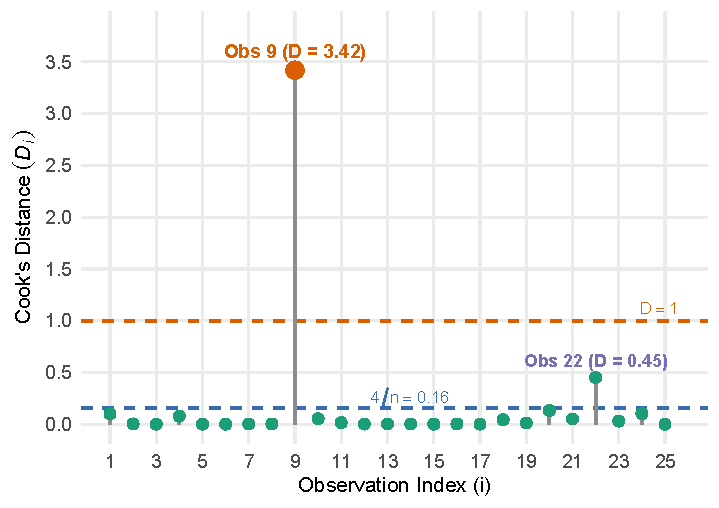
\includegraphics[width=\linewidth]{figures/cooksd-delivery.pdf}}
            \mode<article>{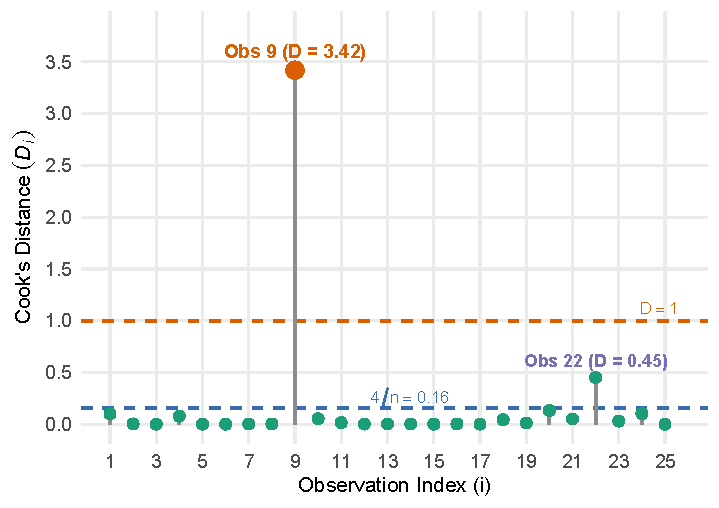
\includegraphics[width=0.8\linewidth]{figures/cooksd-delivery.pdf}}
        \end{column}
    \end{columns}
\end{frame}


\begin{frame}{Residuals Against Leverage}
    \begin{columns}[T]
        \begin{column}{0.38\textwidth}
            \footnotesize
            \begin{itemize}
                \item Each point at $(h_{ii},r_i)$. Red curves: $D_i=0.5$ and $D_i=1$.
                \item $D_i$ depends only on $r_i$ and $h_{ii}$, so one picture shows push, lever arm and influence.
                \item Danger zones: top right and bottom right.
                \item Observation 9 is beyond $D=1$. Observation 22 has high leverage but a moderate residual.
            \end{itemize}
        \end{column}
        \begin{column}{0.62\textwidth}
            \centering
            % Figure: rvl-delivery.pdf (see influence-delivery.R)
            \mode<presentation>{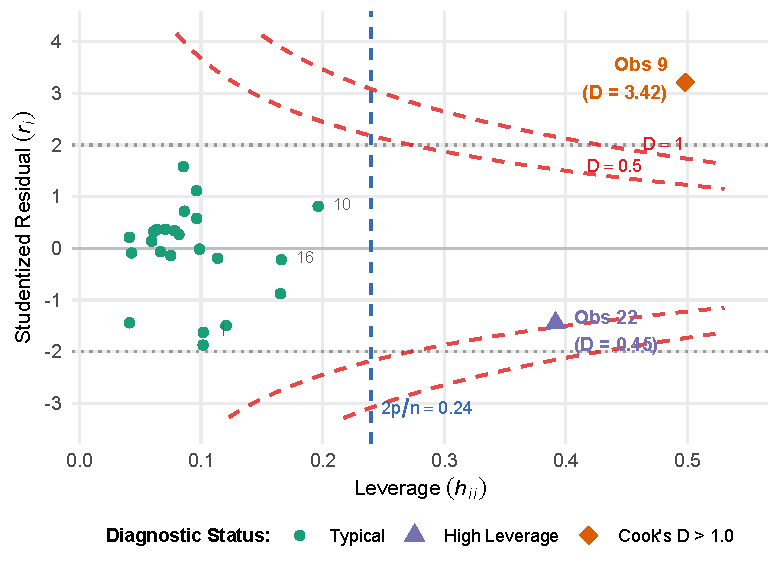
\includegraphics[height=0.78\textheight,width=\linewidth,keepaspectratio]{figures/rvl-delivery.pdf}}
            \mode<article>{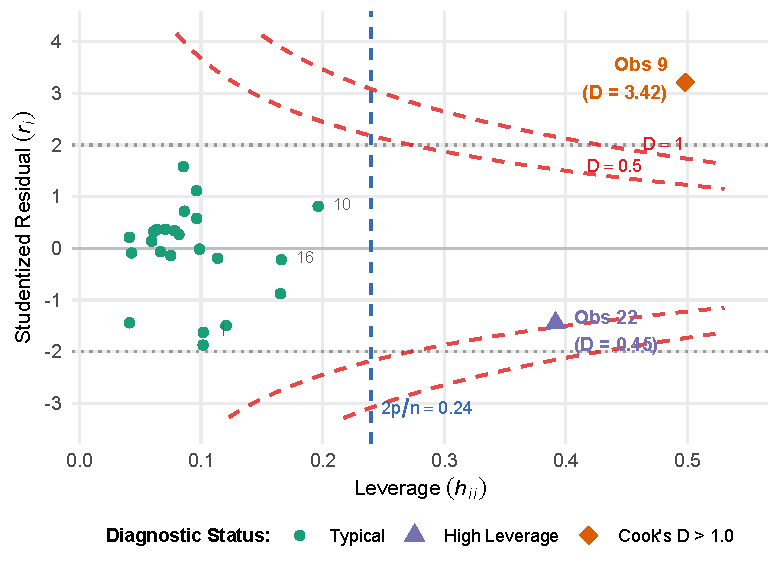
\includegraphics[width=0.8\linewidth]{figures/rvl-delivery.pdf}}
        \end{column}
    \end{columns}
\end{frame}


\subsection{DFBETAS}


\begin{frame}{Which Coefficient Moves? DFBETAS}
    Cook's $D$ says \emph{whether} $\hat{\bbeta}$ moves. Often we care about one coefficient: does observation 9 change the distance effect?
    \[
    \DFBETAS_{j,i}=\frac{\hat\beta_j-\hat\beta_{j(i)}}{\sqrt{S_{(i)}^2\,C_{jj}}},
    \qquad C_{jj}=\bigl[(\bX'\bX)^{-1}\bigr]_{jj}.
    \]
    \begin{itemize}
        \item The change in $\hat\beta_j$, in standard errors. $\DFBETAS=1$: deleting point $i$ moves $\hat\beta_j$ by one standard error.
        \item Sign: positive means $\hat\beta_j$ \emph{falls} when the point is removed, so the point was pulling it up.
        \item Flag $|\DFBETAS_{j,i}|>2/\sqrt n$; $|\DFBETAS_{j,i}|>1$ is large in any sample.
    \end{itemize}
    For each observation there are $p$ values, one per coefficient.
\end{frame}


\begin{frame}{Delivery Time Data: DFBETAS}
    \vspace{-0.5em}
    \begin{center}
        % Figure: dfbetas-delivery.pdf (see influence-delivery.R)
        \mode<presentation>{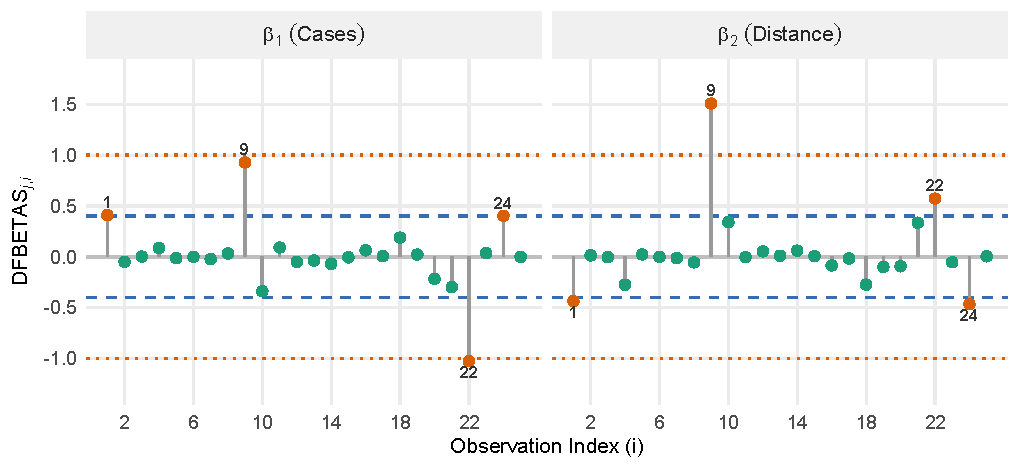
\includegraphics[height=0.5\textheight]{figures/dfbetas-delivery.pdf}}
        \mode<article>{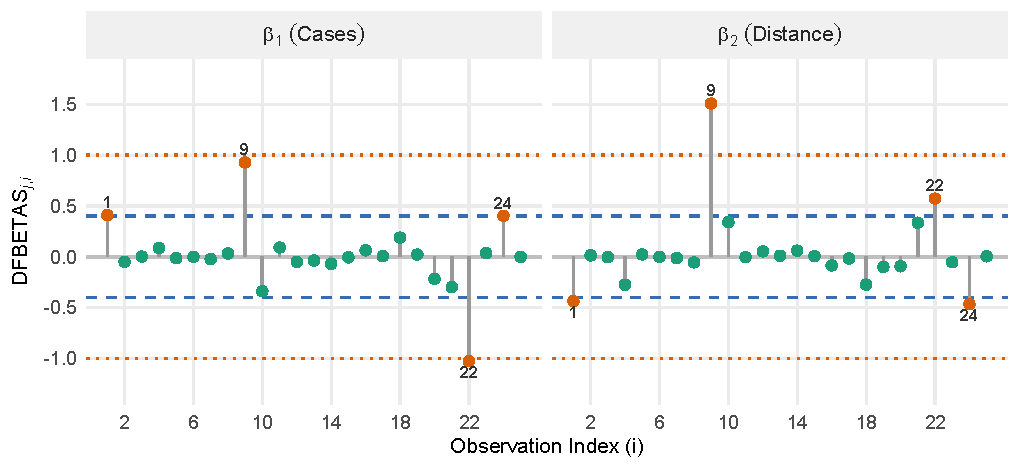
\includegraphics[width=0.9\linewidth]{figures/dfbetas-delivery.pdf}}
    \end{center}
    \vspace{-0.5em}
    \footnotesize
    \begin{itemize}
        \item Cutoff $2/\sqrt{25}=0.4$ (dashed), and $\pm1$ (dotted).
        \item Observation 9: intercept $-2.58$, cases $0.93$, distance $1.51$. It holds the distance slope up and the intercept down.
        \item Observation 22: cases $-1.03$, distance $0.57$. It pulls the cases slope \emph{down}, while observation 9 pulls it up.
    \end{itemize}
\end{frame}


\begin{frame}{Question: Observations 1 and 24}
    \begin{itemize}
        \item Observations 1 and 24 also cross $2/\sqrt n=0.4$ for both slopes ($0.41$, $-0.44$ and $0.41$, $-0.47$). Should they worry us as much as observations 9 and 22?
        \item With $25\times3=75$ DFBETAS values, how many would you expect to cross a cutoff by chance?
    \end{itemize}
    % Answer:
    % - No. They move a slope by less than half a standard error, against 1.5 for observation 9. Their leverage is ordinary (0.10, 0.12) and their R-student is below 2.
    % - The 2/sqrt(n) cutoff is a screen designed to shrink with n so that something gets flagged even in large samples. With 75 values, a few will cross it by chance.
    % - Look at the size of the change and at whether it alters a conclusion, not only at whether a cutoff is crossed.
\end{frame}


\section{Influence on Fitted Values and Precision}


\subsection{DFFITS}


\begin{frame}{DFFITS: Does a Point Pull Its Own Fit?}
    How far does $\hat y_i$ move when observation $i$ is left out, in standard errors of $\hat y_i$?
    \[
    \DFFITS_i=\frac{\hat y_i-\hat y_{(i)}}{\sqrt{S_{(i)}^2\,h_{ii}}}
    =\underbrace{t_i}_{\text{push}}\times\underbrace{\sqrt{h_{ii}/(1-h_{ii})}}_{\text{lever arm}} .
    \]
    \begin{itemize}
        \item The same anatomy as Cook's $D$, with R-student in place of $r_i$. The two are linked by $D_i=\DFFITS_i^2\,S_{(i)}^2/(p\,\MSRes)$ and flag the same kind of point.
        \item $\DFFITS$ has a sign: positive means the point pulls its fitted value up.
        \item Flag $|\DFFITS_i|>2\sqrt{p/n}$; for the delivery data, $2\sqrt{3/25}=0.69$.
    \end{itemize}
\end{frame}


\begin{frame}{Delivery Time Data: DFFITS}
    \begin{columns}[T]
        \begin{column}{0.42\textwidth}
            \small
            \begin{itemize}
                \item Cutoff $\pm0.69$ (dashed).
                \item Observation 9: $\DFFITS_9=4.30$. Without it, the prediction for its own route drops by more than four standard errors.
                \item Observation 22: $\DFFITS_{22}=-1.20$.
                \item Observation 20 ($-0.67$) is just inside.
            \end{itemize}
        \end{column}
        \begin{column}{0.58\textwidth}
            \centering
            % Figure: dffits-delivery.pdf (see influence-delivery.R)
            \mode<presentation>{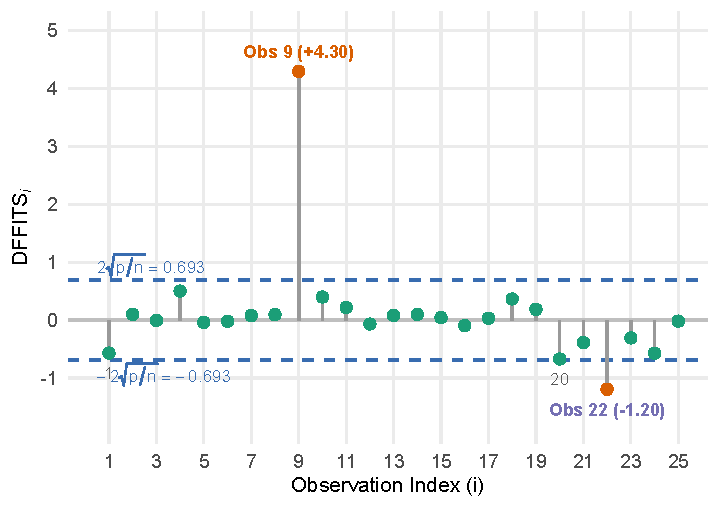
\includegraphics[width=\linewidth]{figures/dffits-delivery.pdf}}
            \mode<article>{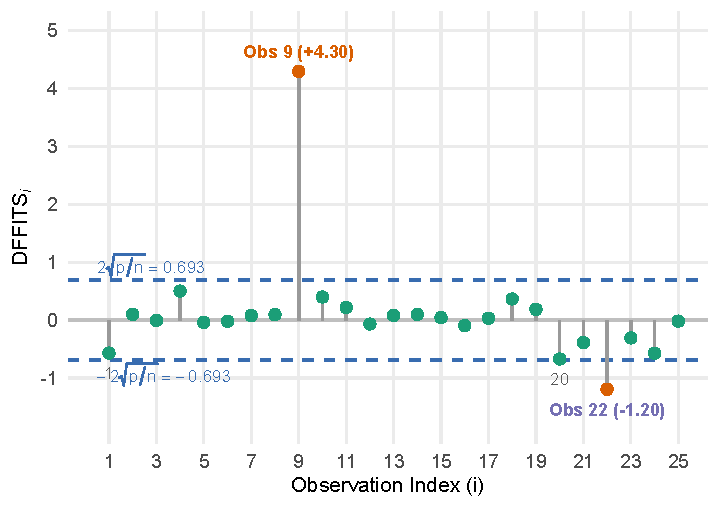
\includegraphics[width=0.8\linewidth]{figures/dffits-delivery.pdf}}
        \end{column}
    \end{columns}
\end{frame}


\begin{frame}{Where Does Observation 9 Matter?}
    Predicted delivery time (min) from the fits with and without observation 9:
    \begin{center}
        \small
        \begin{tabular}{lrrr}
            \toprule
            Route & All 25 & Without 9 & Change \\
            \midrule
            Typical: 10 cases, 500 ft & 25.7 & 24.6 & $-1.1$ \\
            Observation 9's: 30 cases, 1460 ft & 71.8 & 64.5 & $-7.4$ \\
            \bottomrule
        \end{tabular}
    \end{center}
    \begin{itemize}
        \item For a typical route the two fits nearly agree: there are plenty of other routes nearby to pin the prediction down.
        \item At observation 9's own route they differ by more than seven minutes: no other route is anywhere near, so the prediction there rests largely on this one delivery.
        \item A high-leverage point is the data's only witness for its region. That is what makes it valuable, and what makes it dangerous.
    \end{itemize}
\end{frame}


\subsection{COVRATIO}


\begin{frame}{COVRATIO: Does a Point Buy or Cost Precision?}
    The previous measures look at estimates. COVRATIO looks at their \emph{precision}: the size of the confidence region for $\bbeta$ with and without observation $i$.
    \[
    \COVRATIO_i=\frac{\det\bigl[S_{(i)}^2(\bX_{(i)}'\bX_{(i)})^{-1}\bigr]}{\det\bigl[\MSRes(\bX'\bX)^{-1}\bigr]}
    =\frac{\bigl(S_{(i)}^2/\MSRes\bigr)^p}{1-h_{ii}} .
    \]
    \begin{itemize}
        \item The determinant of a covariance matrix (the \emph{generalized variance}) measures the volume of the confidence ellipsoid.
        \item $\COVRATIO_i>1$: without point $i$ the region is larger, so the point \emph{improves} precision.
        \item $\COVRATIO_i<1$: without point $i$ the region is smaller, so the point \emph{degrades} precision.
    \end{itemize}
\end{frame}


\begin{frame}{Two Forces in COVRATIO}
    \[
    \COVRATIO_i=\underbrace{\frac{1}{1-h_{ii}}}_{\text{spread in }\bx\text{: helps}}\;\times\;\underbrace{\left(\frac{S_{(i)}^2}{\MSRes}\right)^p}_{\text{noise in }y\text{: hurts}}
    \]
    \begin{itemize}
        \item \textbf{Leverage helps}: a point far from the centre widens the base of the data, as a longer seesaw is easier to level. In simple regression, $\Var(\hat\beta_1)=\sigma^2/S_{xx}$ shrinks as $S_{xx}$ grows.
        \item \textbf{A large residual hurts}: the point inflates $\MSRes$, so $S_{(i)}^2<\MSRes$ and every standard error grows.
        \item Flag $|\COVRATIO_i-1|>3p/n$. For the delivery data, outside $[0.64,\,1.36]$.
    \end{itemize}
\end{frame}


\begin{frame}{Delivery Time Data: COVRATIO}
    \begin{columns}[T]
        \begin{column}{0.42\textwidth}
            \footnotesize
            \begin{itemize}
                \item Observation 9: $\COVRATIO_9=0.172/0.502=0.34$, where $0.172=(5.91/10.62)^3$. Its leverage would double the precision, but its residual more than cancels that.
                \item Observation 22: $\COVRATIO_{22}=0.850/0.608=1.40$. High leverage and a moderate residual: it \emph{improves} precision.
                \item Observation 16 ($1.37$) is just above the upper limit.            \end{itemize}
        \end{column}
        \begin{column}{0.58\textwidth}
            \centering
            % Figure: covratio-delivery.pdf (see influence-delivery.R)
            \mode<presentation>{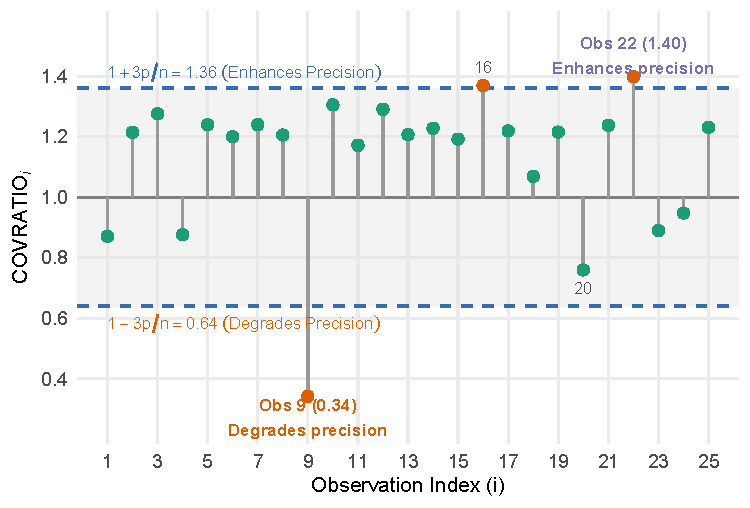
\includegraphics[width=\linewidth]{figures/covratio-delivery.pdf}}
            \mode<article>{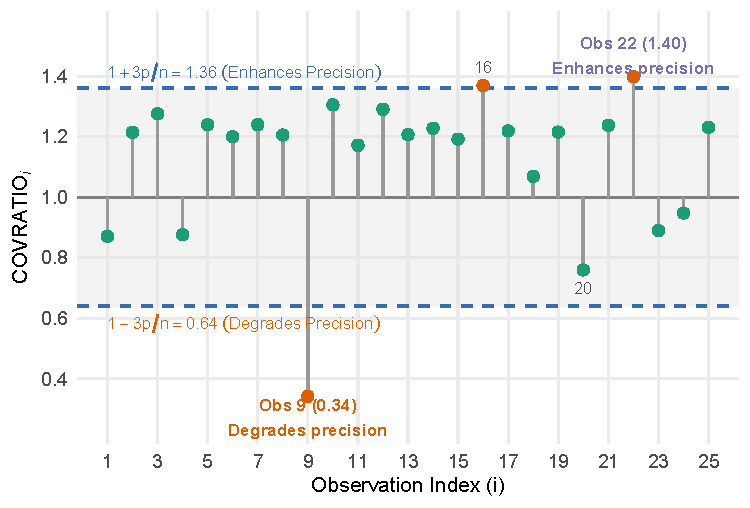
\includegraphics[width=0.8\linewidth]{figures/covratio-delivery.pdf}}
        \end{column}
    \end{columns}
\end{frame}


\begin{frame}{Question: Influential but Helpful?}
    \begin{itemize}
        \item Observation 22 moves the cases slope by one standard error ($\DFBETAS=-1.03$), yet $\COVRATIO_{22}=1.40>1$. Is observation 22 a problem or an asset?
        \item Can a point have a large Cook's $D$ and a $\COVRATIO$ above 1?
    \end{itemize}
    % Answer:
    % - Both at once. It carries real information about large deliveries (it improves precision), but it also changes the estimate, so the conclusion about the cases slope depends on it.
    % - Yes. Cook's D measures how far the estimate moves; COVRATIO measures how the uncertainty changes. A high-leverage point with a moderate residual can do both: shift the estimate and shrink the confidence region.
    % - Influence is not the same as harm. The measures answer different questions.
\end{frame}


\section{Delivery Time Data: Putting It Together}


\begin{frame}{All Measures for the Flagged Points}
    \begin{center}
        \footnotesize
        \setlength{\tabcolsep}{5pt}
        \begin{tabular}{rrrrrrrr}
            \toprule
            $i$ & $h_{ii}$ & $t_i$ & $D_i$ & $\DFFITS_i$ & \multicolumn{2}{c}{$\DFBETAS$} & $\COVRATIO_i$ \\
            & & & & & cases & distance & \\
            \midrule
            Cutoff & 0.24 & 3.53 & 1 & 0.69 & 0.4 & 0.4 & $[0.64,1.36]$ \\
            \midrule
            9 & \textbf{0.498} & \textbf{4.311} & \textbf{3.419} & \textbf{4.296} & \textbf{0.929} & \textbf{1.508} & \textbf{0.342} \\
            22 & \textbf{0.392} & $-1.490$ & 0.451 & $\mathbf{-1.195}$ & $\mathbf{-1.025}$ & \textbf{0.573} & \textbf{1.398} \\
            1 & 0.102 & $-1.696$ & 0.100 & $-0.571$ & \textbf{0.411} & $\mathbf{-0.435}$ & 0.871 \\
            24 & 0.121 & $-1.542$ & 0.102 & $-0.571$ & \textbf{0.405} & $\mathbf{-0.465}$ & 0.948 \\
            20 & 0.102 & $-1.997$ & 0.132 & $-0.672$ & $-0.215$ & $-0.093$ & 0.760 \\
            \bottomrule
        \end{tabular}
    \end{center}
    \begin{itemize}
        \item Bold: beyond the cutoff. Observation 9 fails every check; observation 22 is a high-leverage point that moves the slopes but fits reasonably well.
        \item The others cross at most one screening cutoff, and only just.
    \end{itemize}
\end{frame}


\begin{frame}{Refitting Without the Flagged Points}
    \begin{center}
        \small
        \begin{tabular}{lccc}
            \toprule
            & All ($n=25$) & Without 9 & Without 9 and 22 \\
            \midrule
            $\hat\beta_0$ & 2.341 (1.097) & 4.447 (0.952) & 4.643 (1.126) \\
            $\hat\beta_1$ (cases) & 1.616 (0.171) & 1.498 (0.130) & 1.456 (0.180) \\
            $\hat\beta_2$ (distance) & 0.0144 (0.0036) & 0.0103 (0.0029) & 0.0106 (0.0030) \\
            $\MSRes$ & 10.62 & 5.90 & 6.16 \\
            $R^2$ & 0.960 & 0.949 & 0.907 \\
            \bottomrule
        \end{tabular}
    \end{center}
    Standard errors in parentheses.
    \begin{itemize}
        \item Dropping 9: the distance effect falls by 28\%, and $\MSRes$ almost halves.
        \item Also dropping 22: the coefficients barely move, but the standard errors \emph{grow} ($\COVRATIO_{22}>1$).
    \end{itemize}
\end{frame}


\begin{frame}{Reading the Comparison}
    \begin{itemize}
        \item Observation 9 is the main source of influence. The model without it gives a smaller distance effect and a larger intercept.
        \item $R^2$ falls although the fit gets \emph{better} ($\MSRes$ halves). Observations 9 and 22 stretch the range of $y$ and so inflate $\SST$. A high $R^2$ can be bought by a few extreme points.
        \item Both fits agree that cases and distance matter. The conclusions that change are \emph{how much} distance matters, and predictions for large routes.
        \item Dropping 22 as well costs precision and changes little: there is no reason to remove it.
    \end{itemize}
\end{frame}


\begin{frame}{What Should We Do with Observation 9?}
    \begin{enumerate}
        \item \textbf{Check the record.} Typing error, wrong units, a stopwatch left running? If so, correct it or remove it, and say so.
        \item \textbf{Ask whether it belongs.} A 30-case, 1460-ft delivery may be a different job: several trips, a hand truck, a freight elevator. Then it is from a different population, and the model should not claim to cover it.
        \item \textbf{Ask whether the model is wrong there.} Maybe time does not grow linearly for very large deliveries. One point cannot settle that; more large routes can.
        \item \textbf{Report both fits} when there is no clear answer, and say which conclusions depend on the point.
    \end{enumerate}
    \svspace{0.3em}
    A diagnostic flag is a reason to \emph{investigate}, not a reason to delete.
\end{frame}


\begin{frame}{Deleting Is Not Free}
    \begin{itemize}
        \item \textbf{Overconfidence.} Points that disagree with the model are the ones removed, so $\MSRes$ shrinks and intervals become narrower than the data justify.
        \item \textbf{An endless loop.} After deleting the most extreme point, some other point is the most extreme. Repeated deletion can always produce a ``clean'' data set.
        \item \textbf{Lost information.} Observation 9 is the only route of its size. Without it, every prediction for a large delivery is an extrapolation.
        \item \textbf{Sometimes the outlier is the finding.} An unusual point can reveal a variable that is missing from the model.
    \end{itemize}
\end{frame}


\begin{frame}{An Alternative: Downweighting}
    Deletion is a 0-or-1 decision: a point gets full weight or none.
    \svspace{0.3em}
    \begin{itemize}
        \item \textbf{Robust regression} gives each point a weight between 0 and 1. Points with small residuals get full weight; the weight falls as the residual grows.
        \item Huber's method, for example, counts a residual $e$ as $e^2$ while it is small and only as $|e|$ beyond a threshold. Large residuals still count, but they no longer dominate.
        \item The data decide how much to downweight, so no one has to choose which points to delete.
    \end{itemize}
    \svspace{0.3em}
    Covered in a later lecture, together with weighted least squares.
\end{frame}


\begin{frame}{Question: Two Bad Points Together}
    \begin{itemize}
        \item Suppose two discordant points sit close together, far from the rest of the data. Delete one: what happens to the fit, and to the other point's residual?
        \item Can leave-one-out diagnostics miss both?
    \end{itemize}
    % Answer:
    % - With one deleted, the other still pulls the fit towards the pair, so the deleted point's y does not look surprising: small t_i and small D_i for both. Each one hides the other (masking).
    % - Yes. All measures in this lecture delete one point at a time. Remedies: delete groups of points, look at plots, or use robust regression, which does not let any small group dominate.
\end{frame}


\section{Summary}


\begin{frame}{Diagnostics at a Glance}
    \begin{center}
        \footnotesize
        \setlength{\tabcolsep}{4pt}
        \begin{tabular}{llll}
            \toprule
            Measure & Question it answers & Cutoff & Delivery data \\
            \midrule
            $h_{ii}$ & Is $\bx_i$ far from the others? & $2p/n$ & 9, 22 \\
            $t_i$ (R-student) & Is $y_i$ far from the others' fit? & $t_{\alpha/(2n),n-p-1}$ & 9 \\
            $D_i$ & Does $\hat{\bbeta}$ move as a whole? & 1 (screen $4/n$) & 9 (22) \\
            $\DFBETAS_{j,i}$ & Which coefficient moves? & $2/\sqrt n$ & 9, 22 (1, 24) \\
            $\DFFITS_i$ & Does $\hat y_i$ move? & $2\sqrt{p/n}$ & 9, 22 \\
            $\COVRATIO_i$ & Does precision change? & $|\cdot-1|>3p/n$ & 9 ($-$), 22 ($+$) \\
            \bottomrule
        \end{tabular}
    \end{center}
    All are computed from one fit, using $e_i$, $h_{ii}$ and $S_{(i)}^2$; no refitting is needed.
\end{frame}


\begin{frame}{Key Takeaways}
    \begin{itemize}
        \item Outlier (unusual $y$), high leverage (unusual $\bx$) and influence (changes the fit) are different things. Influence needs both a push and a lever arm.
        \item Leverage $h_{ii}$ is the distance of $\bx_i$ from the centre of the data, measured along the data cloud; its fair share is $p/n$.
        \item R-student keeps the point out of its own yardstick and has an exact $t_{n-p-1}$ distribution; test the largest with a Bonferroni cutoff.
        \item Cook's $D$, DFBETAS, DFFITS and COVRATIO measure what deleting a point does to $\hat{\bbeta}$, to one $\hat\beta_j$, to $\hat y_i$ and to precision.
        \item Flagged points call for investigation. Delete only with a reason from outside the data, and report both fits when in doubt.
    \end{itemize}
\end{frame}
